\section{Experiments}\label{sec:exp}

The goal for this section is twofold. First, we would like to compare
the bandwidth consumption of \MSWave{} with some baseline and
state-of-the-art approaches. Second, we intend to provide some discussions
on a variety of scenarios and configurations.

\subsection{Data Description and Experiment Setup}\label{subsec:setup}

We use one real data set and one synthetic data set in our experiments. For the real data set,
we choose a public dataset recording the daily average temperature of
300 cities around the world acquired from the temperature data archive
of the University of Dayton. The data from each city is considered as a
time series with 2048 data points. 
For the synthetic data set, we use the same random walk data model used in \cite{Rakthanmanon:2012:SMT}. Each time series is generated by the random walk whose every step size is a normal distributed random number with mean=0 and standard deviation=1. There are 12,500 time series of length 12,500 generated.
After selecting $|Q|$ time series as
the reference set, the candidate time series are chosen from the remaining
time series and are equally distributed to the $m$ machines.

We consider five frameworks: (i) CP, which is the Concurrent
Processing baseline~\cite{PAP01DPS} described in
Section~\ref{sec:intro}, but generalized to $|Q| > 1$ by sending the
whole query set at the beginning; (ii) PRP, which is the Probabilistic
Processing method~\cite{PAP01DPS} mentioned in Section~\ref{sec:intro}, 
but again generalized to $|Q| > 1$ in a straightforward manner;
(iii) \LeeWave-M{}, as discussed in Section~\ref{subsec:limitations};
(iv) \MSWave-S{} (Fig.~\ref{fig:mswave-s}); and 
(v) \MSWave-L{} (Fig.~\ref{fig:mswave-l}).

We compare the total bandwidth cost for these five frameworks in a
distributed environment simulated in MATLAB. We study the influences 
on the bandwidth cost of the size of the reference set $|Q|$, the time series 
length $T$, the number of machines $m$, and the $k$ for $k$NN/$k$FN.
The total bandwidth
cost is the summation of all data transmitted between the server and
other local machines. Note that in this simulation framework,
practical issues such as the overheads of message headers, packet losses,
retransmissions, etc.~were not considered.

There are two strategies we employ to choose the time series that
comprise the instances in a query set $Q$.
For the \emph{analogous reference set}, we choose one time series randomly
and then choose its closest $|Q|$-1 neighbors to form $Q$; thus the queries
in $Q$ are highly similar.
For the \emph{random reference set}), we choose $|Q|$ time series at random;
thus the queries in $Q$ are likely to be dissimilar.

\begin{figure}[tb]
\centering
\subfigure[random reference set] {
\label{fig:1(a)}
%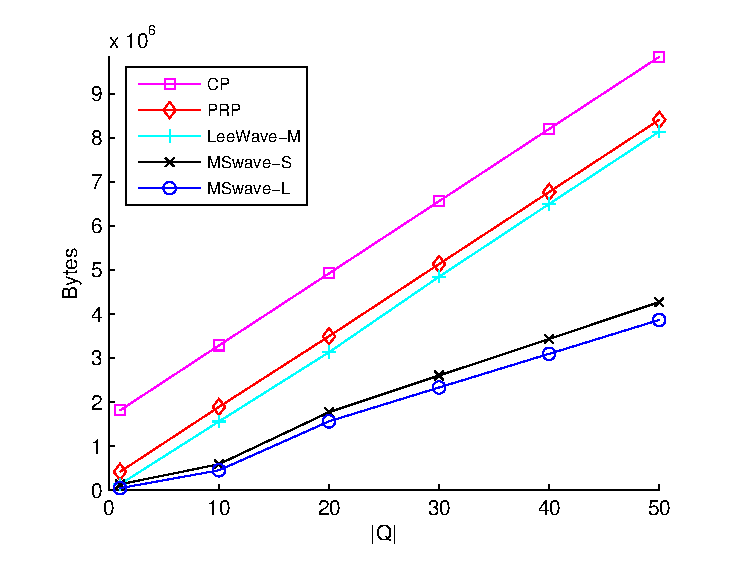
\includegraphics[scale=0.3]{1(a).eps}
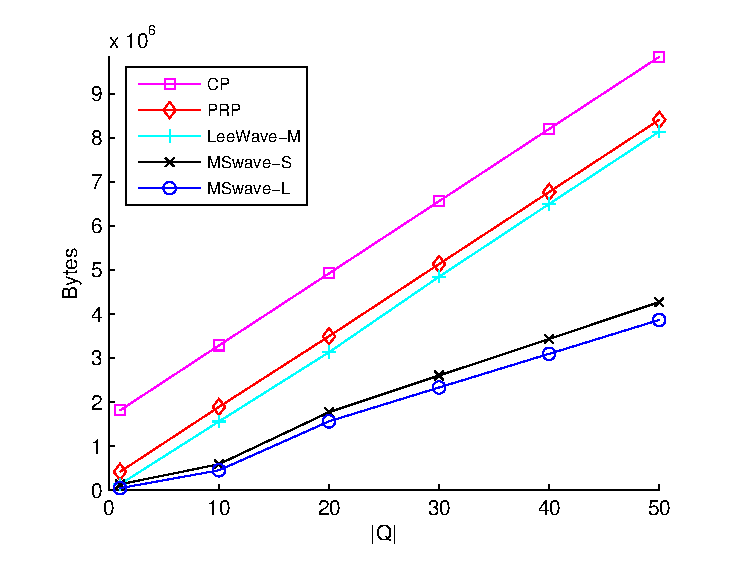
\includegraphics[scale=0.5]{1(a).eps}
}
\subfigure[analogous reference set] {
\label{fig:1(b)}
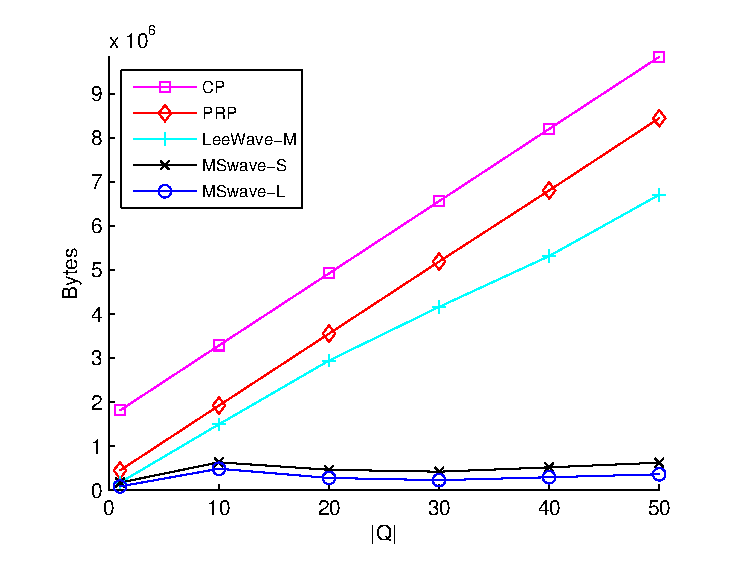
\includegraphics[scale=0.5]{1(b).eps}
}
\vspace{-0.05in}
\caption{\label{fig:1}
Comparison between frameworks given two kinds of query sets, $T$=1024, 
$k$=10, $m$=20, $d_{com}$, and $k$FN}
\vspace{-0.05in}
\end{figure}

\begin{figure*}[t!]
\centering
\subfigure[$k$=10, $|Q|$=10,  $d_{com}$,  $k$FN] {
\label{fig:2(a)}
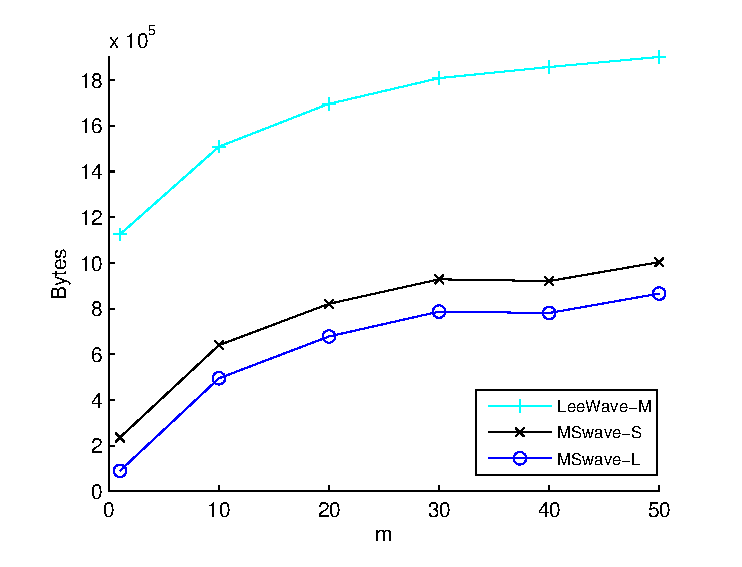
\includegraphics[scale=0.45]{2(a).eps}
}
\hspace{0.1cm}
\subfigure[$k$=10, $|Q|$=10, $d_{sin}$, $k$NN] {
\label{fig:2(b)}
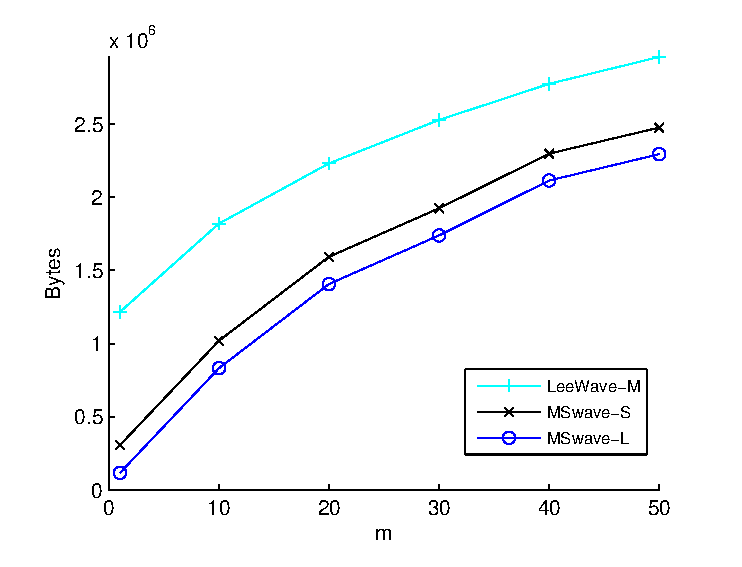
\includegraphics[scale=0.45]{2(b).eps}
}
\hspace{0.1cm}
\subfigure[$k$=10, $m$=20,  $d_{com}$, $k$FN] {
\label{fig:2(c)}
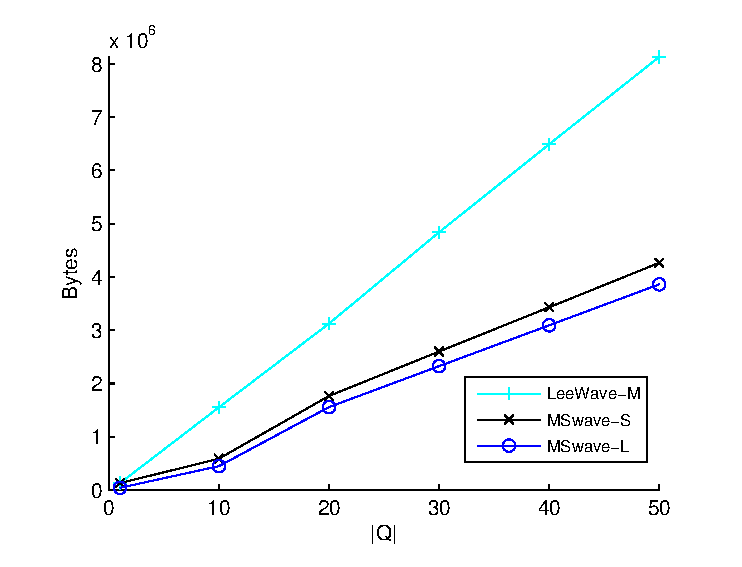
\includegraphics[scale=0.45]{2(c).eps}
}
\hspace{0.1cm}
\subfigure[$k$=10, $m$=20, $d_{sin}$,  $k$NN] {
\label{fig:2(d)}
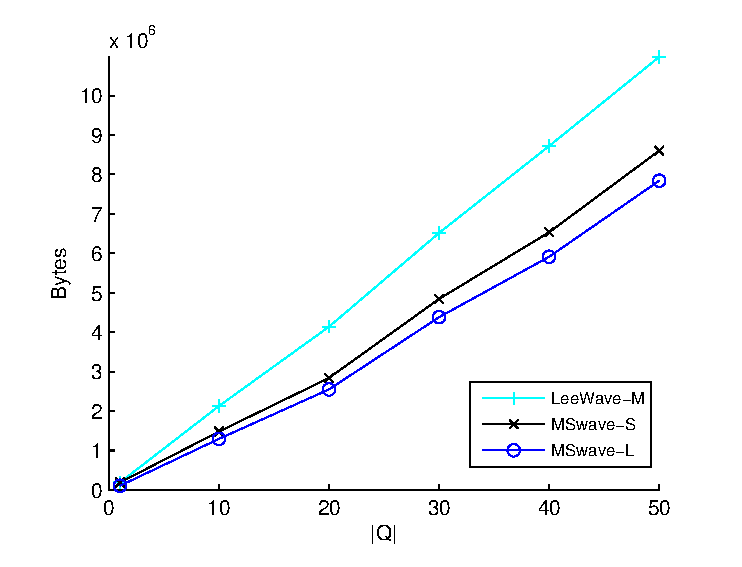
\includegraphics[scale=0.45]{2(d).eps}
}\hspace{0.1cm}
\subfigure[$m$=20, $|Q|$=10, $d_{com}$,  $k$FN] {
\label{fig:2(e)}
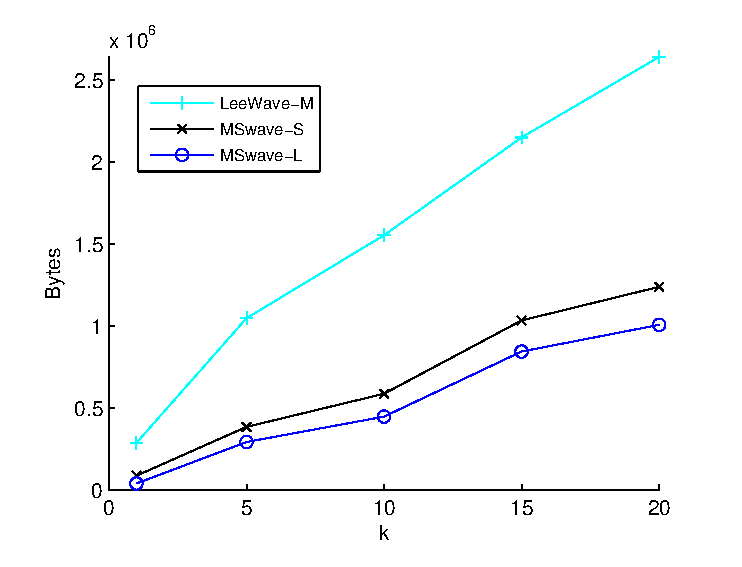
\includegraphics[scale=0.45]{2(e).eps}
}\hspace{0.1cm}
\subfigure[$m$=20, $|Q|$=10,  $d_{sin}$, $k$NN] {
\label{fig:2(f)}
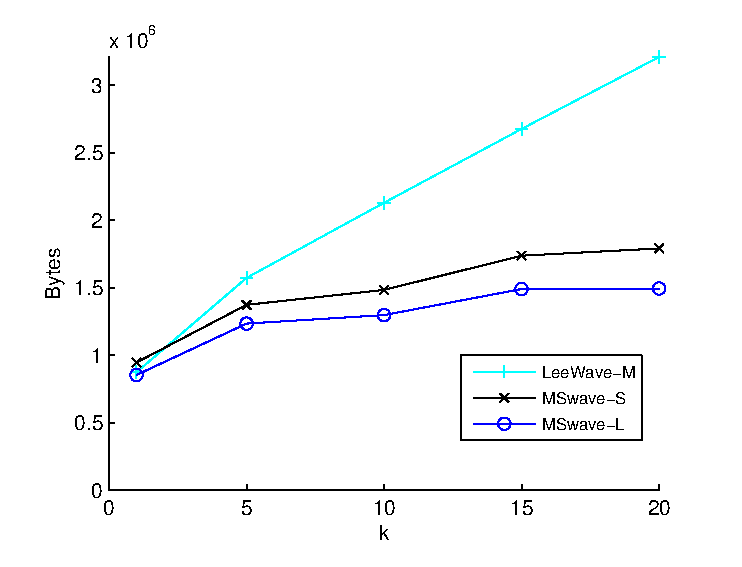
\includegraphics[scale=0.45]{2(f).eps}
}
\vspace{-0.05in}
\caption{Comparison between frameworks given the random reference set, 
$T$=1024.}
\label{fig:2}
\end{figure*}

\subsection{Comparison on Real Data}

\textbf{Comparing all five frameworks.}
Fig.~\ref{fig:1} shows a comparison of the total bandwidth consumption
of all five frameworks, for both the random reference set (Fig.~\ref{fig:1}(a))
and the analogous reference set (Fig.~\ref{fig:1}(b)).
Both plots show that the \MSWave{} frameworks outperform the
other frameworks significantly. We also find the slopes of \MSWave{}
frameworks are
less steep than the slopes of the others, highlighting the benefits of
using Eq.~\eqref{eq:avg_LB}$-$\eqref{eq:com_UB} for pruning. For
analogous reference sets, we even find that the bandwidth costs of the 
\MSWave{} frameworks do not increase significantly when $|Q|$ increases. 
This can be explained as follows. When the reference time series are 
similar, the distance to any one of the reference time series is very 
close to the distance to the whole reference set. This holds regardless of 
whether $d_{avg}$, $d_{sin}$, or $d_{com}$ is chosen. Therefore, in
the early levels of the protocol, we already obtain enough information
to estimate the true distance, which leads to more effective
pruning. On the other hand, for the random reference set, because the
distances to each reference vary a lot, it is generally required to
send many levels of coefficients to be able to accurately estimate the
true distance to determine the $k$NN/$k$FN neighbors, thus consuming
more bandwidth.

\textbf{Comparing \MSWave-L{}, \MSWave-S{} and \LeeWave-M{}.}  Next,
Fig.~\ref{fig:2} highlights the comparison of \MSWave-S{}, \MSWave-L{},
and \LeeWave-M{} in total bandwidth consumption. 
We choose $k$NN for $d_{sin}$ (Fig.~\ref{fig:2(b)}, \ref{fig:2(d)},
\ref{fig:2(f)}) and $k$FN for $d_{com}$ (Fig.~\ref{fig:2(a)},
\ref{fig:2(c)}, \ref{fig:2(e)}) because, as argued in
Section 2.3, these are the only two feasible cases for \LeeWave-M{}.
The figure shows that the performance of \MSWave-L{}
is clearly better than \MSWave-S{}, while both are much better than
\LeeWave-M{} in all configurations.
 
Figs.~\ref{fig:2(a)} and \ref{fig:2(b)} present the results while
varying the number of machines $m$ from 1 to 50. The figures show that
increasing $m$ does not change the performance differences
significantly.  Figs.~\ref{fig:2(c)} and \ref{fig:2(d)} study the
performance impact of the size of reference set $|Q|$, which is varied 
from 1 to 50.  The figures show that the \MSWave-L{}'s bandwidth
savings over \LeeWave-M{} increases as $|Q|$ increases. On
the other hand, while \MSWave-L{}'s bandwidth savings over \MSWave-S{}
also increases as $|Q|$ increases, the increase is less significant.
The savings increases because, the larger the reference
set is, the more values \MSWave-S{} has to send from the local machines to
the server, as analyzed in Section~\ref{subsec:analysis}. Finally,
Figs.~\ref{fig:2(e)} and \ref{fig:2(f)} examine the impact of $k$ on 
the performance, with $k$ varying from 1 to 20.
It is not hard to reason that the difference
between \LeeWave-M{} and \MSWave-L{} in bandwidth consumption
increases as $k$ increases because \LeeWave-M{}'s overhead grows linearly with
$k$. We can also see that the difference between \MSWave-L{} and
\MSWave-S{} increases slightly as $k$ becomes larger. The larger $k$ is,
the fewer candidate series are pruned early, and based on our discussion in
Section~\ref{subsec:analysis}, the gap becomes larger when there are more 
candidate series still remaining.

\textbf{Comparing the upper bounds in Eq.~\eqref{eq:upper-bound} and
Eq.~\eqref{eq:single-UB}.} Table \ref{tbl:bound} compares our new upper
bound in Eq.~\eqref{eq:single-UB} to the upper bound derived in \LeeWave{} 
in Eq.~\eqref{eq:upper-bound}. The
parameters in this experiment are $d_{avg}$ in $k$FN, random reference
set, $T$=1024, $k$=10, $m$=150, and $|Q|$=10. The new bounds
are slightly lower, which makes them better for pruning, although
the improvement is quite small.

\begin{table*}[tb]
\centering
\caption{New bound (Eq.~\eqref{eq:single-UB}) vs old bound (Eq.~\eqref{eq:upper-bound}) , $T$=1024, $k$=10, $m$=150, $|Q|$=10}
\label{tbl:bound}
\vspace*{0.05in}
\begin{tabular}{|l|l|l|l|l|l|l|l|l|l|l|l|}
\hline
step & 1 & 2 & 3 & 4 & 5 & 6 & 7 & 8 & 9 & 10 & 11 \\ \hline
new bound & 150.0 & 150.0 & 148.9 & 137.3 & 53.9 & 32.5 & 24.8 & 19.8 & 15.2 & 11.5 & 8.0 \\ \hline
old bound & 150.0 & 150.0 & 150.0 & 139.1 & 62.4 & 33.7 & 26.0 & 20.3 & 15.6 & 11.5 & 8.0 \\ \hline
\end{tabular}
\vspace{0.1in}
\end{table*}

\begin{figure*}[t]
\centering
\subfigure[Bandwidth consumption under different $|Q|$ and $m$] {
\label{fig:Y3(a)}
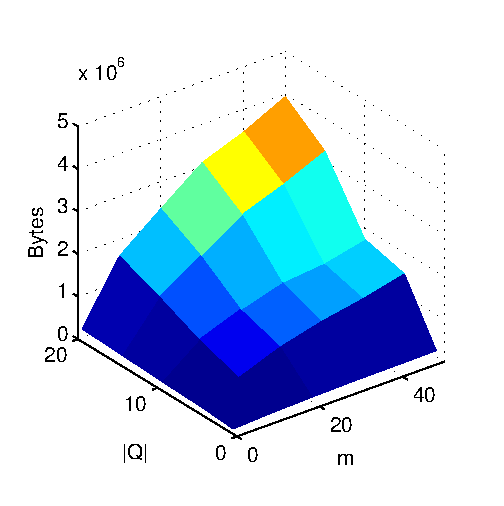
\includegraphics[scale=0.45]{Y3(a).eps}
}
\hspace{0.1cm}
\subfigure[Number of candidate machines in each level, $m$=50] {
\label{fig:Y3(b)}
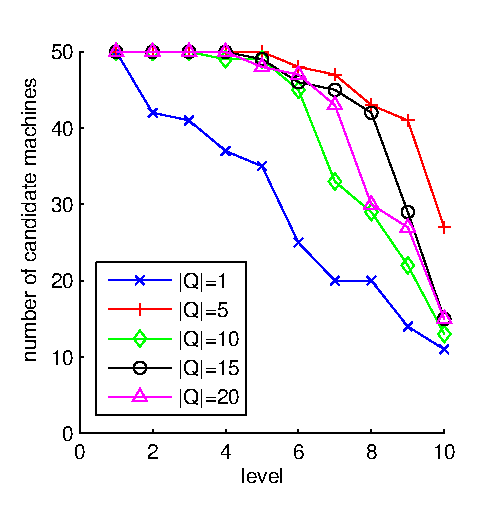
\includegraphics[scale=0.45]{Y3(b).eps}
}
\hspace{0.1cm}
\subfigure[Bandwidth consumption under different $|Q|$ and $m$] {
\label{fig:Y4(a)}
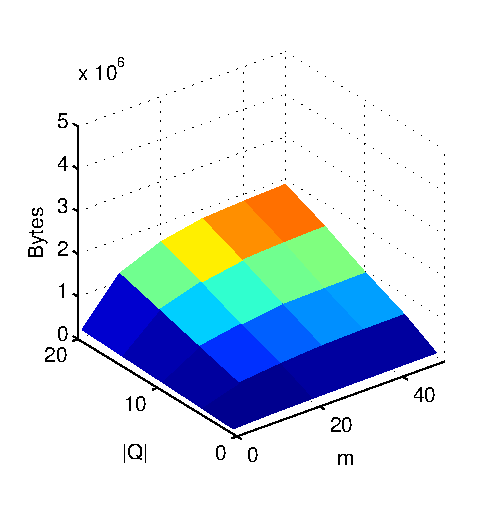
\includegraphics[scale=0.45]{Y4(a).eps}
}
\hspace{0.1cm}
\subfigure[Number of candidate machines in each level, $m$=50] {
\label{fig:Y4(b)}
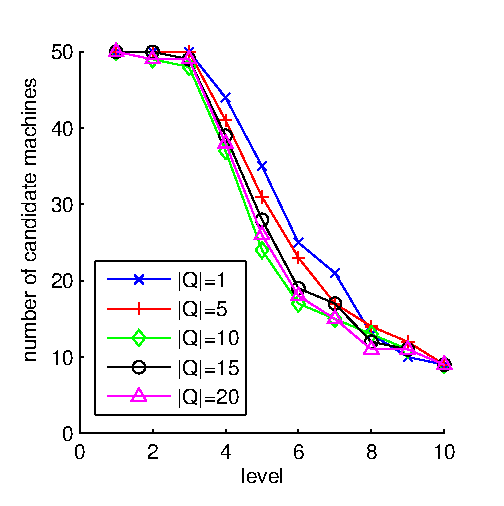
\includegraphics[scale=0.45]{Y4(b).eps}
}
\vspace{-0.05in}
\caption{Results of $k$NN queries using \MSWave-L{} with $d_{avg}$ for either
random reference sets ((a),(b)) or analogous reference sets ((c),(d)), 
$T$=1024, $k$=10}
\label{fig:Y3Y4}
\vspace{-0.1in}
\end{figure*}

\subsection{Sensitivity Analysis of \MSWave-L{} on Real Data}

The previous results have shown that \MSWave-L{} outperforms the other
frameworks.  To gain additional insights into its performance, we present
a further sensitivity analysis for \MSWave-L{} in this section.
%We discuss how the bandwidth usage
%of \MSWave-L{} would be influenced by variables such as the size of the reference set, the type of reference set, and the distance measurements.

\begin{figure*}[tb]
\centering
\subfigure[$d_{avg}$] {
\label{fig:Y5(a)}
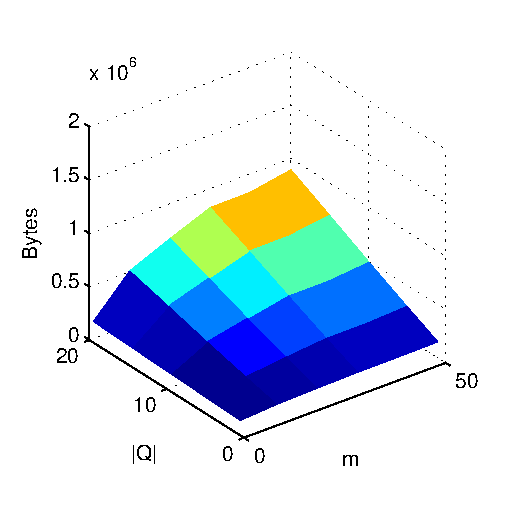
\includegraphics[scale=0.5]{Y5(a).eps}
}
\hspace{0.1cm}
\subfigure[$d_{sin}$] {
\label{fig:Y5(b)}
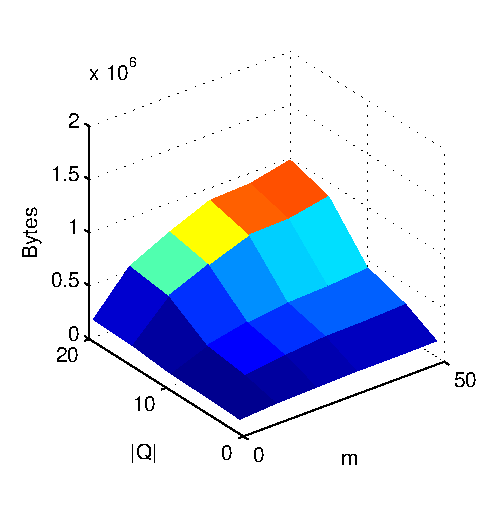
\includegraphics[scale=0.5]{Y5(b).eps}
}
\hspace{0.1cm}
\subfigure[$d_{com}$] {
\label{fig:Y5(c)}
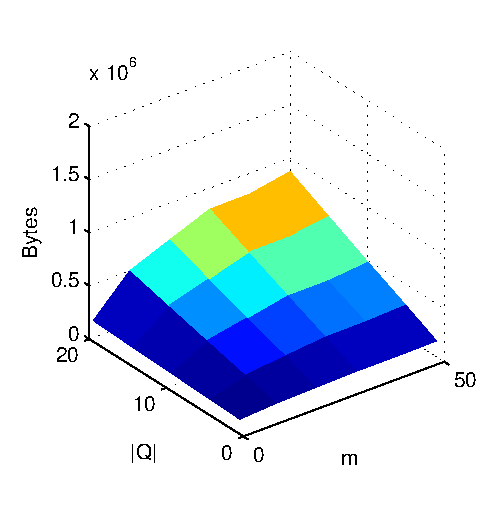
\includegraphics[scale=0.5]{Y5(c).eps}
}
\vspace{-0.05in}
\caption{Results for $k$FN queries with different linkage distances given analogous reference sets, $T$=1024, $k$=10}
\label{fig:Y5}
\end{figure*}

\textbf{Sensitivity to query set size and number of machines.}  First,
we examine the impact of the size of the reference set $|Q|$ and the
number of machines $m$ on the bandwidth consumption for finding $k$NN
under $d_{avg}$. In this experiment, we fix $k$=10 and $T$=1024, while
$|Q|$ is varied from 1 to 20 and $m$ is varied from 1 to 50, and we
consider both the random and analogous reference sets.
Figs.~\ref{fig:Y3(a)} (random) and \ref{fig:Y4(a)} (analogous) show
that the bandwidth consumption generally increases as $|Q|$ increases. 
An exception occurs for the random reference sets, where the bandwidth 
consumption of $|Q|$ = 10 is smaller than $|Q|$=5. By looking into
Fig.~\ref{fig:Y3(b)} we find that the pruning power of $|Q|$=10 was
also better than that of $|Q|=5$. This is because when the size of
the reference set increases from $|Q|$=5 to $|Q|$=10, certain reference
time series that are close to many candidates were included in the set,
which enables \MSWave-L{} to quickly prune many candidates. A similar
effect can be seen in Fig.~\ref{fig:Y4(b)} for the analogous reference
sets. In this case, the bandwidth consumption of \MSWave-L{} does not
increase too much with the growth of $|Q|$, which matches our
discussion in the previous section.

\textbf{Sensitivity to distance measure.} 
Finally, we examine the influence of the different distance
measures. We compare the three distance measures using analogous
reference sets to do $k$FN queries when $T$=1024, $k=10$, $|Q|$ is
varied from 1 to 20 and $m$ is varied from 1 to 50. As shown in
Fig.~\ref{fig:Y5}, we can see little difference between the measures
in terms of bandwidth consumption. The reason is that when the patterns in the
reference set are very similar to each other, the distances between
an arbitrary candidate series and each reference series is very
close. Thus, their $d_{avg}$, $d_{sin}$, and $d_{com}$ should be
similar. As a result, the bounds obtained in every round are similar,
and so are the final results. On the other hand, for random reference
sets, we find no consistent patterns among the three distance
measures. The bandwidth consumption indeed depends on how the reference
set is chosen.


\subsection{Comparison on Large-scale Synthetic Data}

We conclude our experimental study with a comparison of the five
frameworks on the large-scale synthetic data set discussed in
Section~\ref{subsec:setup}.  The purpose is to compare their bandwidth
consumption when the number of time series and the length of each time
series are much larger, namely, both are increased to 12,500.  Recall
that both \MSWave{} and \LeeWave-M{} can work when the time series
pattern length is not a power of 2. We also increase the total number
of machines to 500.

Fig.~\ref{fig:11(a)} shows the bandwidth consumption of all frameworks
using a logarithmic scale under the parameter settings $T=$12,500,
$k=30$, $m=500$, $d_{com}$, $k$FN, and the random reference set,
varying $|Q|$ from 10 to 50. The bandwidth savings for \MSWave-L{} and 
\MSWave-S{} are even more dramatic, about 1 to 2 orders of magnitude,
compared to CP, PRP, and \LeeWave-M{}. \MSWave{}'s advantage is fairly
consistent across the range of $|Q|$.  In addition, we also
observe the gap between \MSWave-L{} and \MSWave-S{} increases as
$|Q|$ increases, again agreeing with the analysis in Eq.~\eqref{eq:bandwidthsaved}.

Finally, Fig.~\ref{fig:11(b)} focuses in on \MSWave-L{}, the best
framework, and shows the effectiveness of its candidate pruning at
each level for the large-scale data set. The parameter settings are
the same as the prior experiment. The significant drop in the number
of candidate machines when only the coefficients of the top-half
levels are passed is the main reason for its significant bandwidth
savings. The results in this section demonstrate the added advantage of
\MSWave-L{} when $m$ is large and much greater than $k$.

\begin{figure}[tb]
\centering
\subfigure[Bandwidth consumption of all frameworks] {
\label{fig:11(a)}
%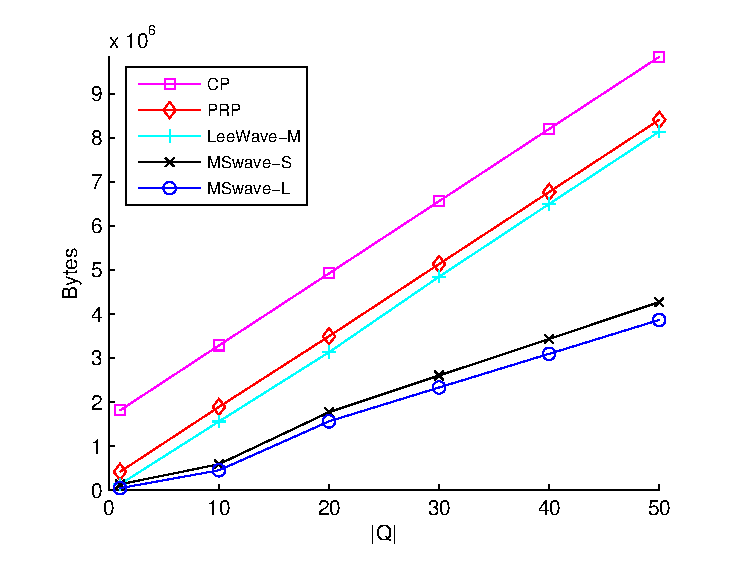
\includegraphics[scale=0.3]{1(a).eps}
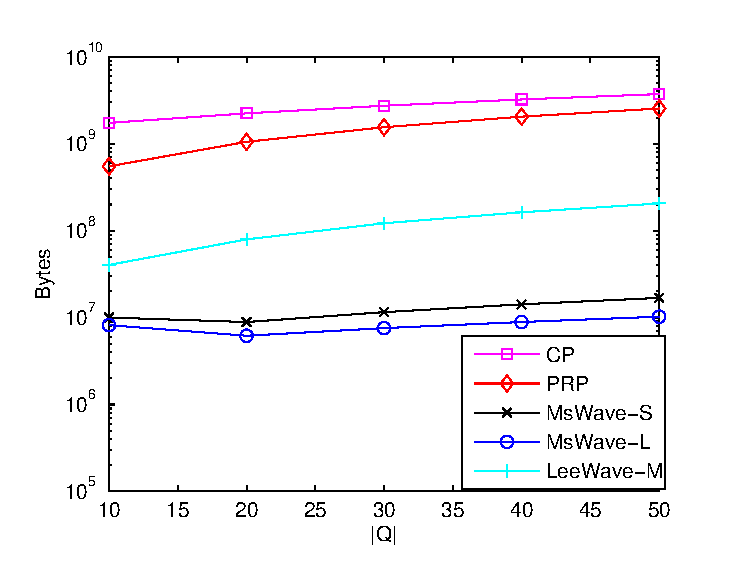
\includegraphics[scale=0.5]{5compare_log.eps}
}
\subfigure[Number of candidate machines in each level of \MSWave-L{}.] {
\label{fig:11(b)}
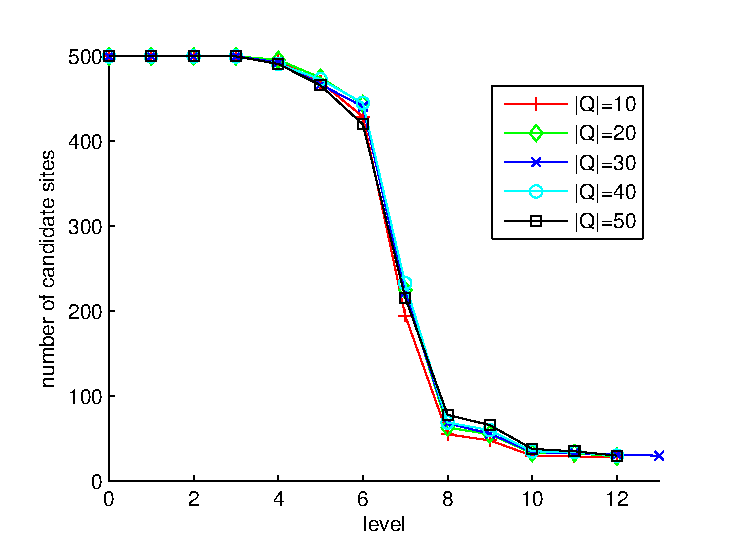
\includegraphics[scale=0.5]{rand_site_v2.eps}
}
\vspace{-0.05in}
\caption{\label{fig:11}
Experiments on synthetic data with random reference set, $T$=12500, $k$=30, $m$=500, $d_{com}$, $k$FN.}
\vspace{-0.05in}
\end{figure}


